\chapter{Beschreibung des Versuchs}

Dieser Versuch befasst sich mit der Einrichting eines Cisco Switches, sowie
eines Cisco Routers und einer Einf�hrung in den Cisco Packet Tracer.

\section{Versuchsaufbau}\label{Aufbau}

\begin{figure}[h!]
\centering
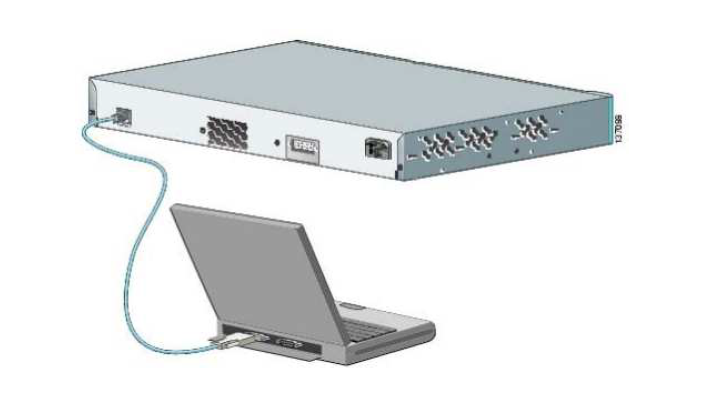
\includegraphics[width=0.7\textwidth]{Graphics/Switch.PNG}
\caption{Versuchsaufbau- Computer mit Switch verbinden}
\label{fig:switch}
\end{figure}

\begin{figure}[h!]
\centering
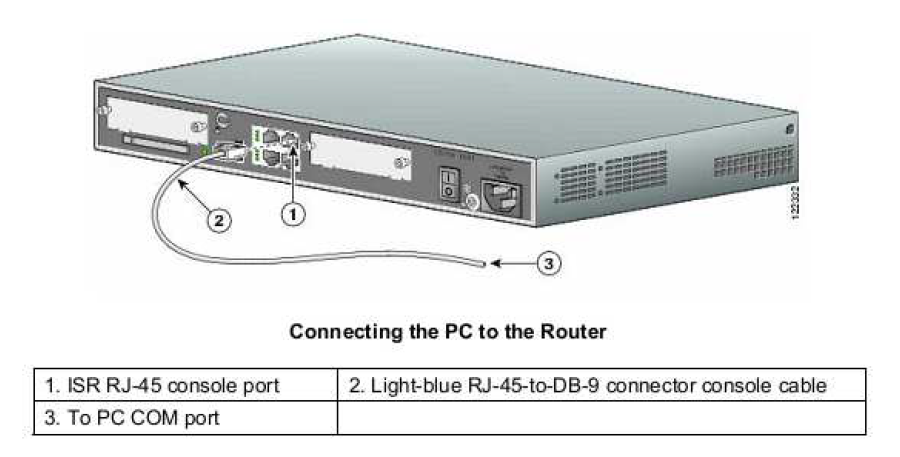
\includegraphics[width=0.7\textwidth]{Graphics/Router.PNG}
\caption{Versuchsaufbau - Computer mit Router verbinden}
\label{fig:router}
\end{figure}

\subsection{Komponenten}

\begin{itemize}
  \item 1 Cisco 2811 Router
  \item 1 Cisco 2960 Switch
  \item Windows PC mit einem terminal emulation program (HyperTerminal)
  \item RJ45-to-DB9 connector console Kabel
\end{itemize}

\section{Versuchsdurchf�hrung}

Im ersten Teil des Versuchs wird ein Initial Setup des Cisco 2960 Switchs
durchgef�hrt. Der zweite Teil besch�ftigt sich mit dem Initial Setup des Cisco
2811 Routers.\\Im dritten Teil werden show commands genutzt, um bestimmte
Informationen aus dem Router System zu erhalten.\\Abschlie�end besch�ftigt sich
der vierte Teil mit einer Einf�hrung in den Packet Tracer.


\section{Versuchsziel}

Der Laborversuch dient dazu einen ersten Einblick mit dem Umgang von Switches
und Router zu erlangen und einen groben �berblick �ber den Cisco Packet Tracer
schaffen.
